\section{The ATLAS experiment at the Large Hadron Collider}\label{sec:atlas}
Exploring the nature of the Higgs particle requires collision energies on the \qty[]{}{TeV} scale. The \ac{lhc} is currently the most powerful particle accelerator making it the best available facility for studying the Higgs particle. This section relies heavily on \citep{aad2008atlas}.

\subsection{The Large Hadron Collider}
The \ac{lhc} is a circular proton proton collider with \qty[]{27}{km} circumference with a center-of-mass energy of $\sqrt{s}=\qty[]{13}{TeV}$. The two anticyclic proton beams are actually bunches containing $10^{11}$ protons that are brought to collisions at several points of the ring for the experiments performed at the \ac{lhc}. A measure of how tightly particles are packed in these bunches is the instantaneous luminosity and is characteristic to the collider
\begin{equation}
    L=\frac{1}{\sigma}\frac{\dint{N}}{\dint{t}}.
\end{equation}
It can be read as particle interactions per unit time and area. The area understood as the interaction cross-section of a particular process. The total recorded number of collision events is then with the integrated luminosity 
\begin{equation}
    N=\sigma\cdot\int L dt=\sigma\cdot L_\mathrm{int}.
\end{equation}
For the full run 2 dataset used in this thesis the integrated luminosity for events good for physics analysis is \qty[]{140.1}{fb^-1}\citep{DAPR-2021-01}. When bunches are collided not only one but rather several proton-proton interactions are measured. Methods to disentangle the different interactions in the detector improved over time so the mean number of interactions also called pile up increased during the data taking period as can be seen in figure \ref{fig:pileup}.
\begin{figure}
    \centering
    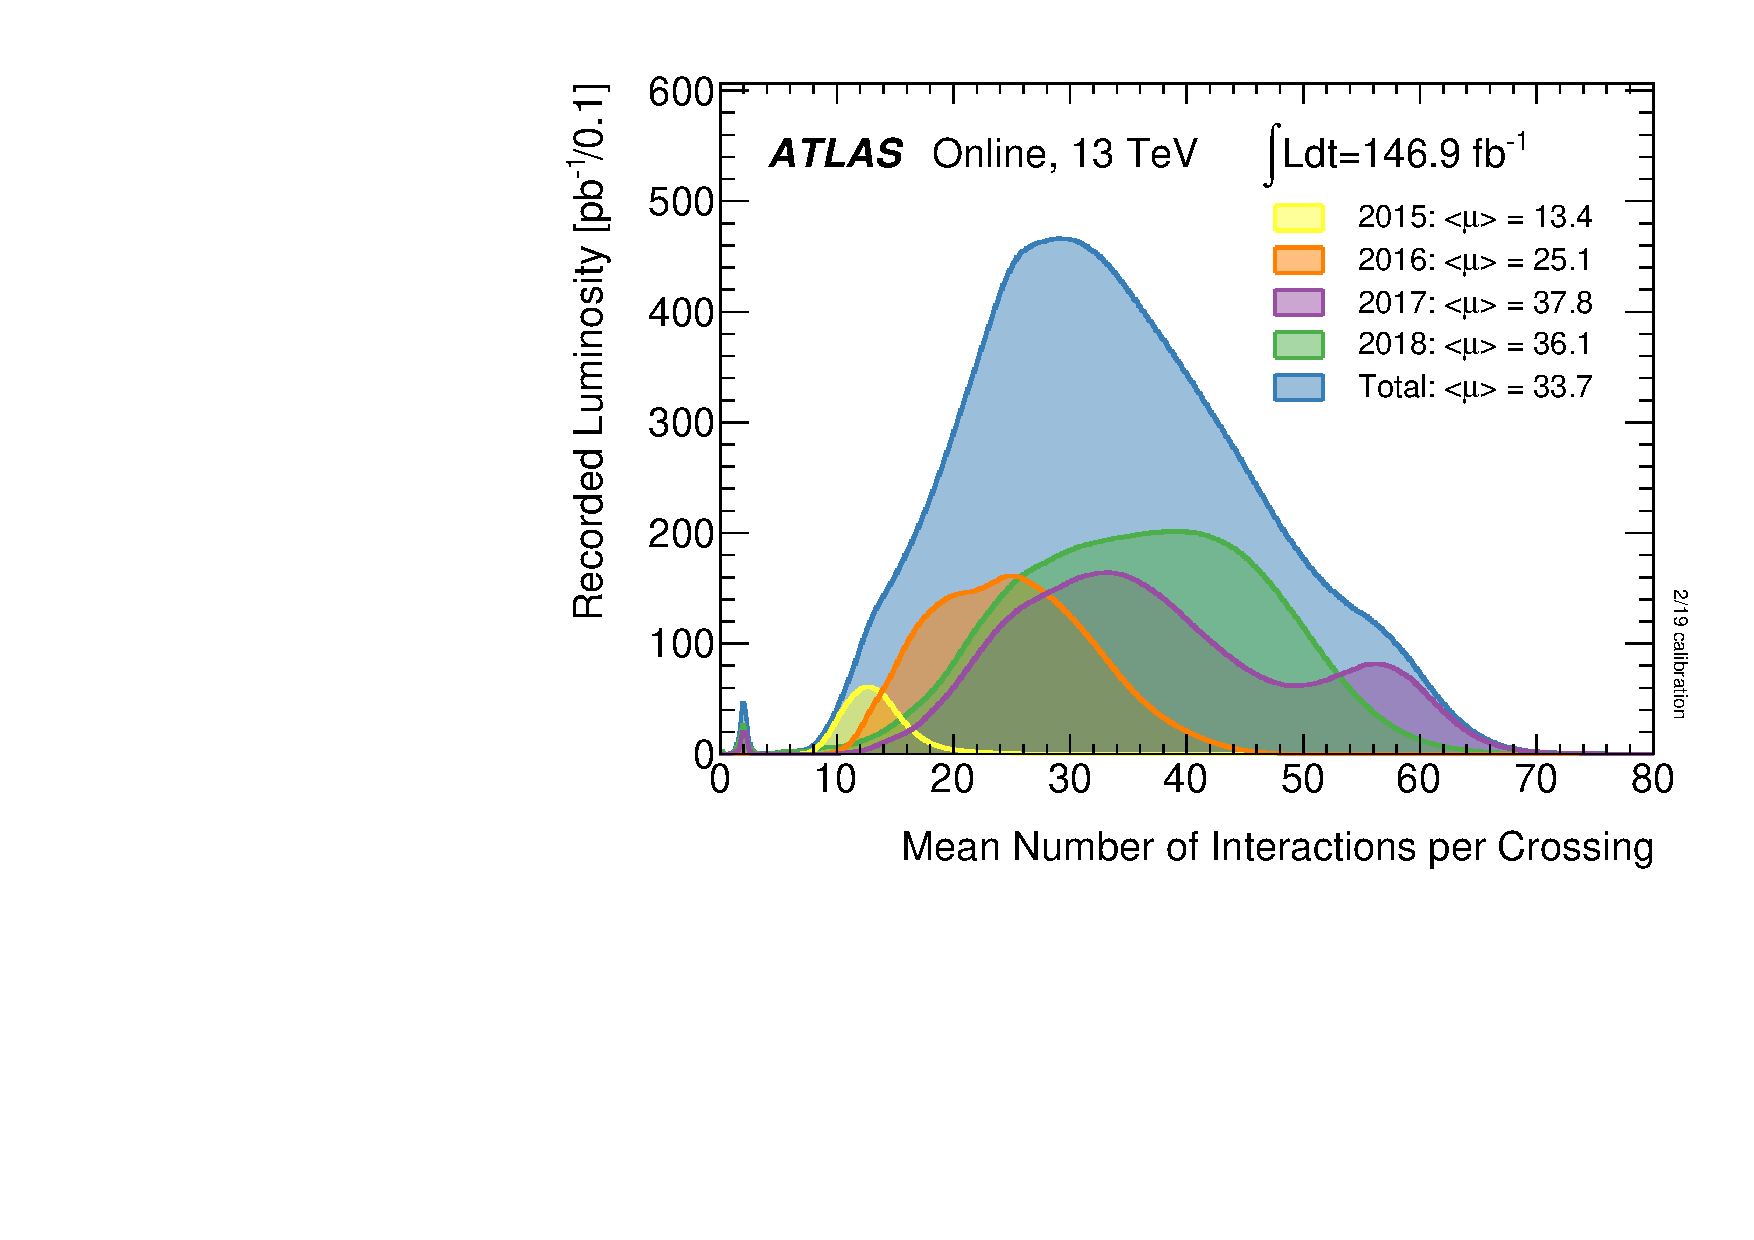
\includegraphics[width=0.5\textwidth]{mu_2015_2018}
        \caption[]{Pile up profiles for run 2 data taking periods \citep{pileup}.}
    \label{fig:pileup}    
\end{figure}

\subsection{ATLAS detector}
where experiments are conducted and one of them is the \ac{atlas} experiment.


\begin{figure}
    \centering
    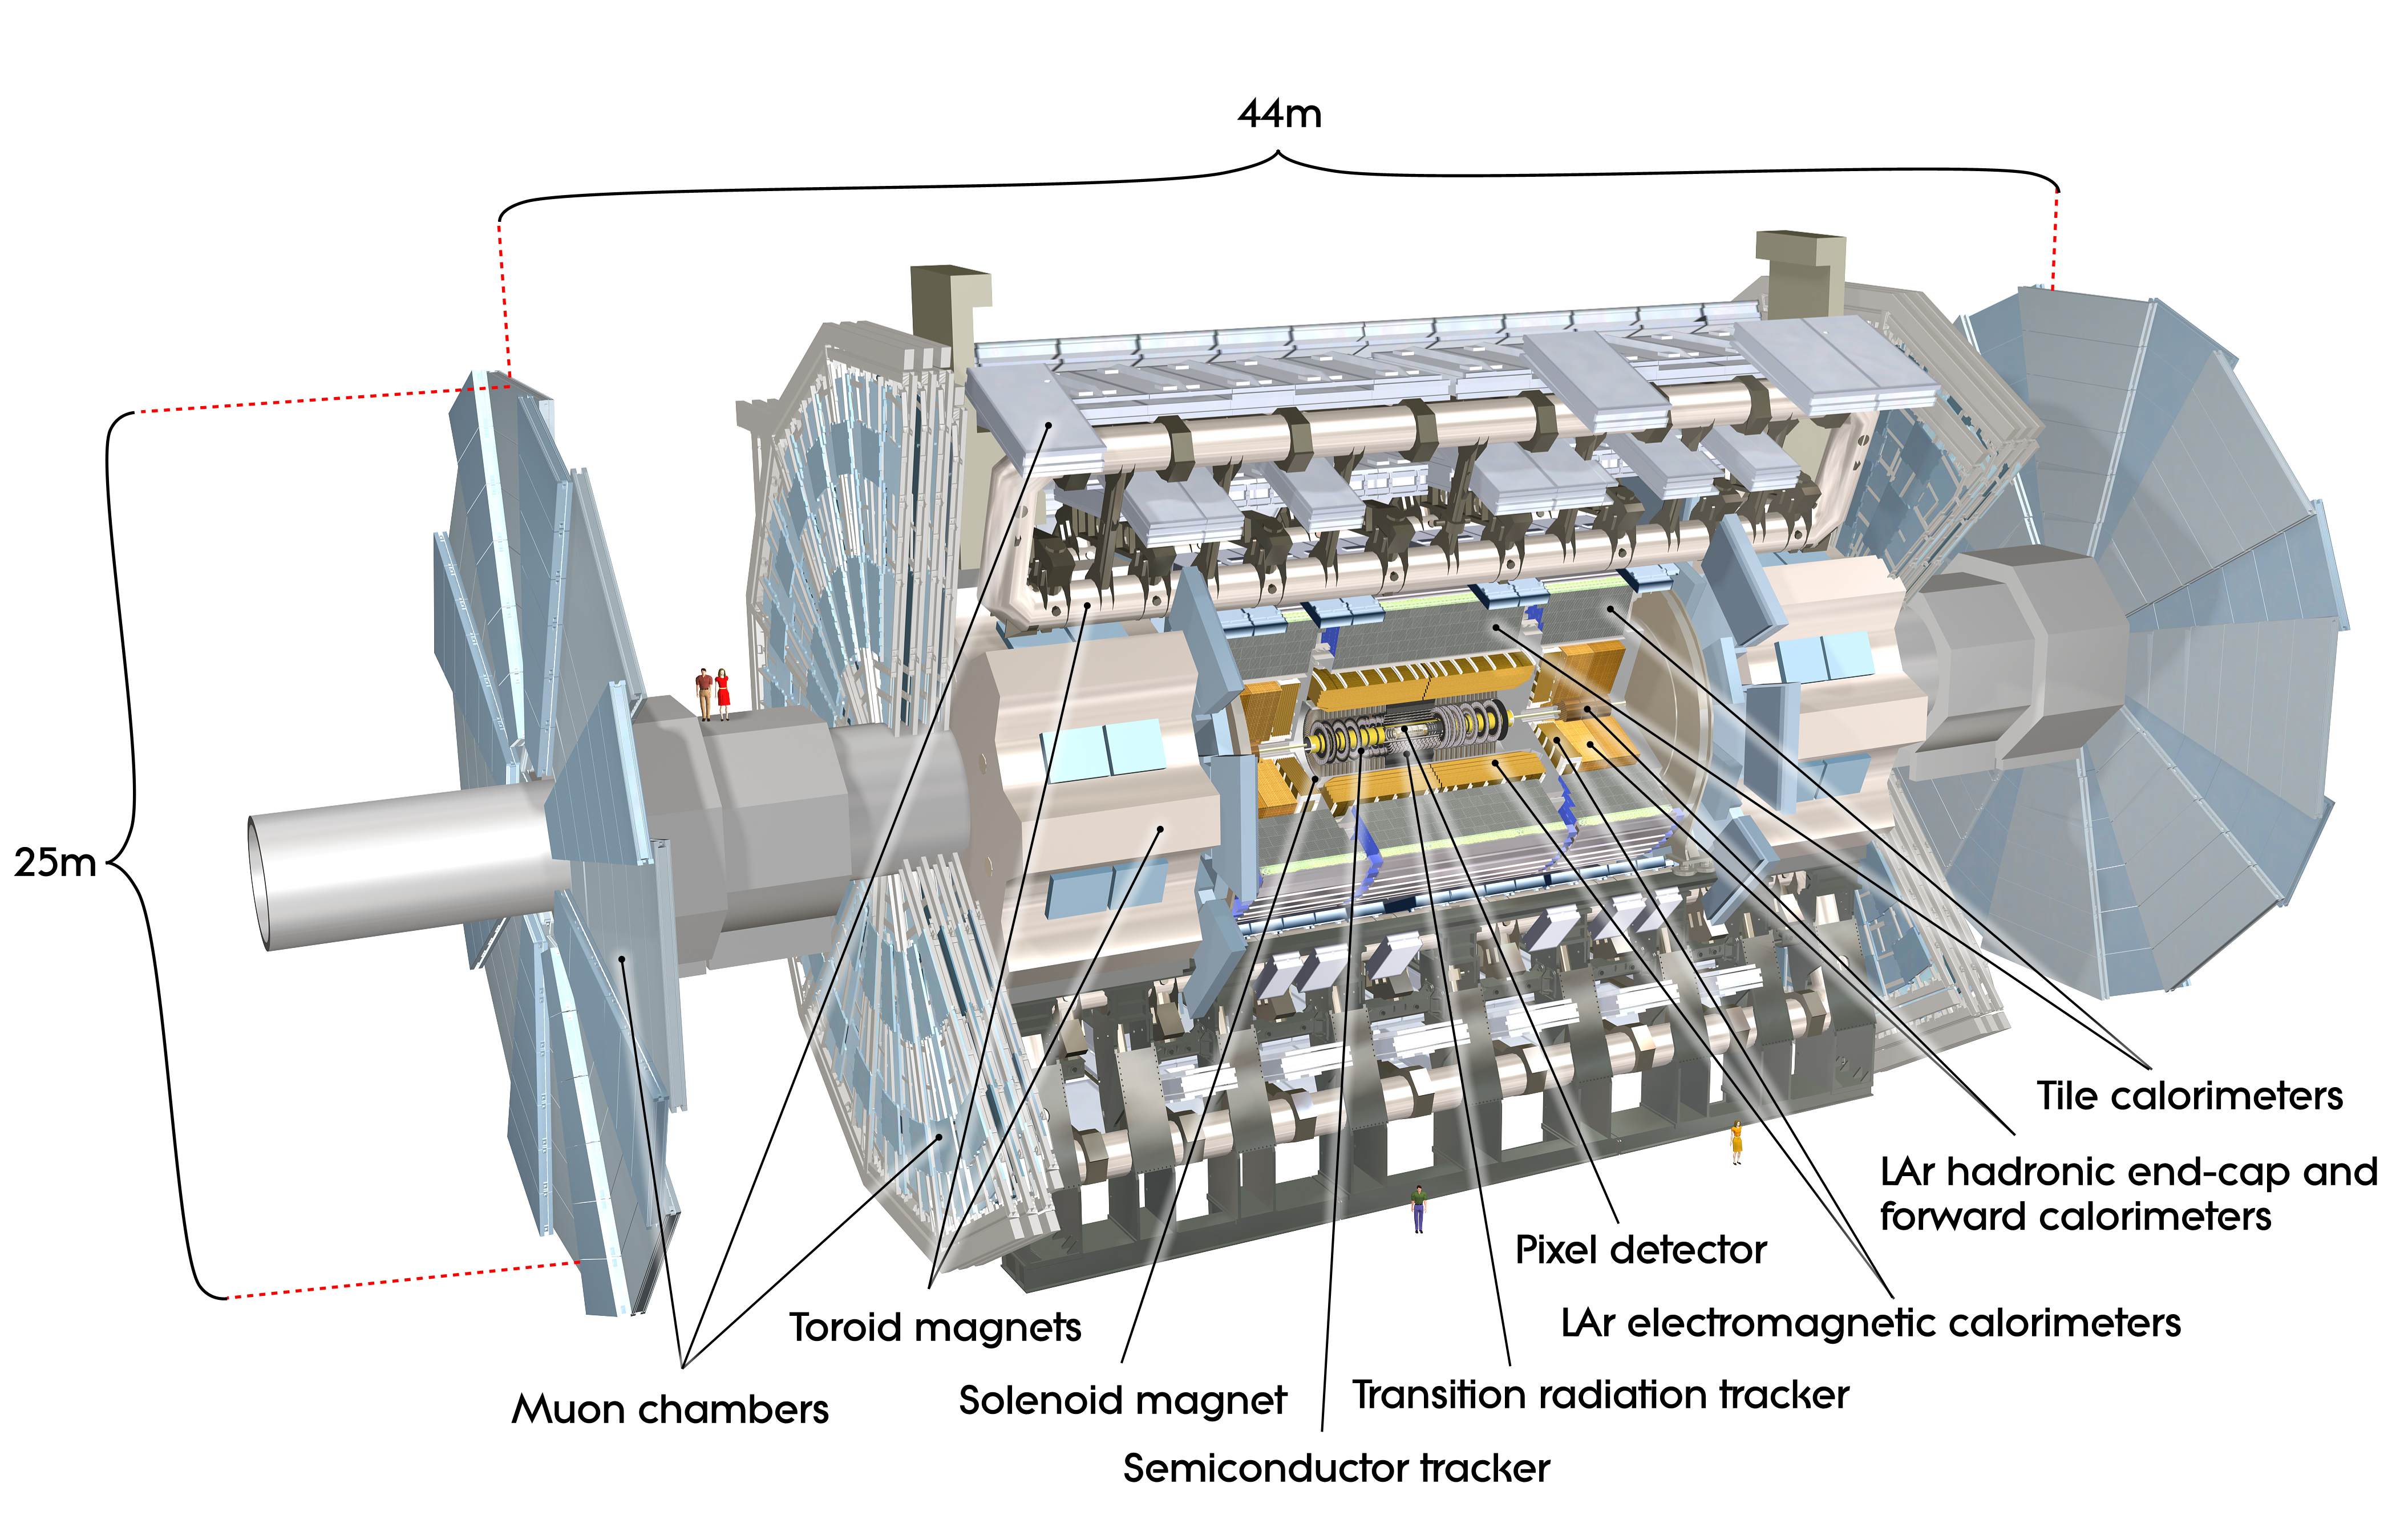
\includegraphics[width=1\textwidth]{atlas_detector}
        \caption[]{}
    \label{fig:atlas_detector}    
\end{figure}


